\documentclass[thesis.tex]{subfiles}

\begin{document}
\iffulldocument\else
	\chapter{Introduction}
\fi

\section{Historical Background}

Solitary waves are localized disturbances that maintain their shape as they propagate at a constant velocity. The first recorded observation of this phenomenon in nature is the Russell's famous ``great solitary wave''. In 1834, the Scottish engineer John Scott Russell observed a ``large solitary elevation'' which arose when a barge stopped suddenly on the Union Canal near Edinburgh (see \cref{fig:canalwave} for a recreation of this experiment in 1995). He was subsequently able to recreate the solitary wave experimentally, both in canals and in a wave tank in his backyard.  
\begin{figure}
\begin{center}
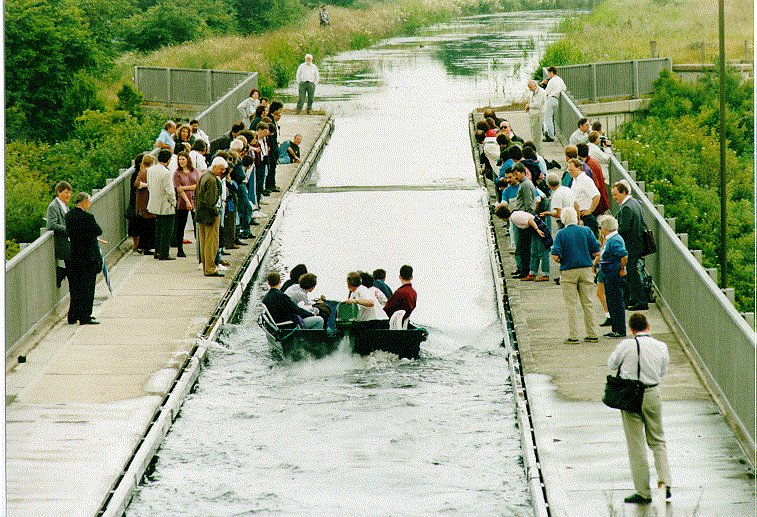
\includegraphics[width=7cm]{images/intro/solitonHW.jpg}
\caption{Recreation of solitary wave experiment on the Union Canal, 12 July, 1995 \cite{Nature1995} }
\label{fig:canalwave}
\end{center}
\end{figure}

Although Russell published his results in 1845 \cite{russell1845}, his research was not well-received in the scientific community. The prominent mathematicians George Airy and George Stokes both rejected his work, as it did not agree with their results. The first mathematical theory to support the Russell's observations was published by Boussinesq in 1872 \cite{Boussinesq1872}. Boussinesq opens his paper by vindicating Russell, stating that ``tous les ing{\'e}nieurs conaissent les belles exp{\'e}riences de J. Scott Russell... sur la production et la propagation des ondes solitaires'' [every engineer knows the great experiments of J. Scott Russell on the production and propagation of solitary waves]. In 1877, Boussinesq introduced an equation to describe solitary wave phenomena \cite{boussinesq1877essai}. This equation was rediscovered in 1985 by Diederek Korteweg and Gustav de Vries \cite{KdVoriginal} and is now known as the Korteweg-de Vries (KdV) equation. More recently, solitary waves have found applications in diverse fields, including fiber optics \cite{Taylor1992}, molecular systems \cite{Davydov1985}, Bose-Einstein condensates \cite{Panos2008BEC}, and ferromagnetics \cite{Kosevich1998}.

\section{Korteweg-de Vries equation}

The Korteweg-de Vries (KdV) equation is a prototypical model of an equation which admits solitary wave solutions. The equation derived by Korteweg and de Vries \cite{KdVoriginal} to describe wave propagation in a rectangular canal is  
\[
\frac{d \eta}{dt} = \frac{3}{2} \sqrt{\frac{g}{l}}
\frac{\partial}{\partial x}
\left( \frac{1}{2} \eta^2 + \frac{2}{3} \alpha \eta + \frac{1}{3} \sigma \frac{\partial^2 \eta}{\partial x^2}\right),
\]
where $\eta$ is the displacement above the surface, and remaning quantities are physical constants. It can be derived from the Euler equation for nonviscous, incompressible fluids, together with the appropriate boundary conditions and the assumption of irrotational flow \cite{SolitonPhysics}. With an appropriate change of variables, the KdV equation can be put into the more tractable form
\begin{equation}\label{KdV3}
\partial_t \phi + \partial_x^3 \phi - 6 \phi \partial_x \phi = 0
\end{equation}
This equation has been extensively studied since its introduction \cite{miles1981,drazin1989solitons,SolitonPhysics}, and many variants have been proposed. For wavespeed $c > 0$, an exact solitary wave solution to the KdV equation can be obtained by an inverse scattering transform.
\[
\phi (x,t)=-{\frac {c}{2}}\,\mathrm {sech} ^{2}\left({{\sqrt {c}} \over 2}(x-c\,t-a)\right),
\]
where $a$ is an arbitrary constant. The KdV equation also has another class of exact solutions which are periodic in nature. There are termed cnoidal waves, since they are expressed in terms of the Jacobi elliptic function $cn$ \cite{drazin1989solitons}. The cnoidal waves have sharper peaks and flatter troughs than ordinary sine waves. Images of both classes of solutions for water waves are shown in \cref{fig:waterwave}.
\begin{figure}
\begin{center}
\begin{tabular}{cc}
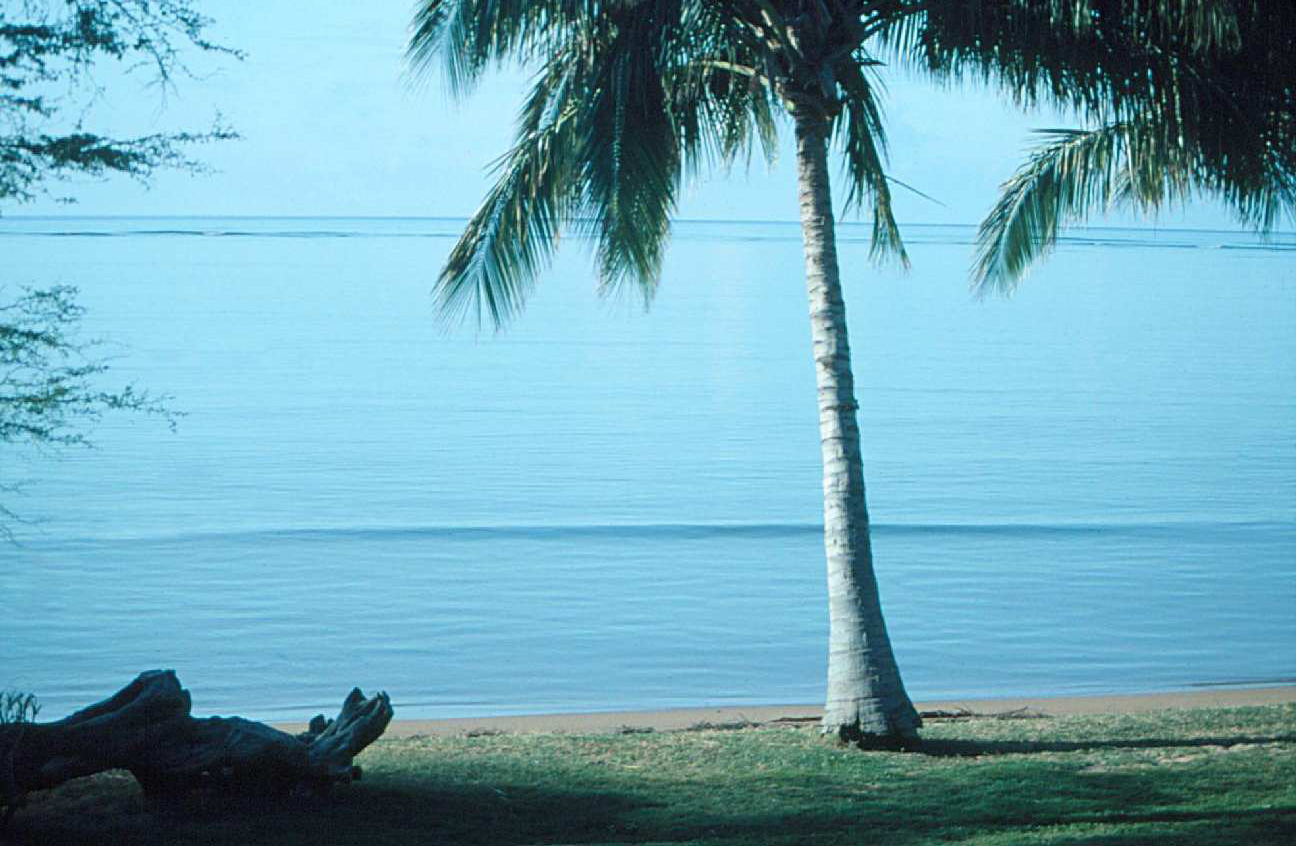
\includegraphics[width=7cm]{images/intro/beach.jpg} &
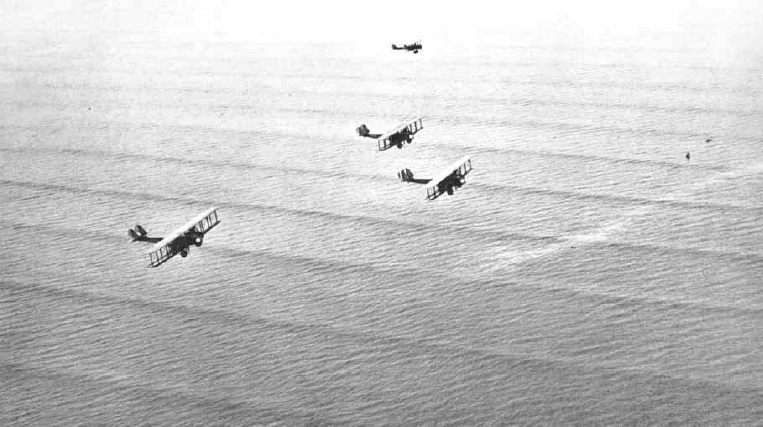
\includegraphics[width=7cm]{images/intro/cnoidal.jpg}
\end{tabular}
\caption{Solitary wave observed off the coast of Hawaii \cite{ANDRIOPOULOS2009} (left), periodic solitary waves observed by US Army bombers near the Panama coast in 1933 (right) }
\label{fig:waterwave}
\end{center}
\end{figure}

Since solitary waves maintain their shape as they propagate at a constant velocity, they are equilibrium solutions to an approprate nonlinear PDE when written in a co-moving frame. For KdV, for example, a solitary wave with wavespeed $c$ is a solution to the third order ODE 
\begin{equation}\label{KdV3eq}
\partial_x^3 \phi - c \partial_x \phi - 6 \phi \partial_x \phi = 0
\end{equation}
Since solitary waves are also localized, we can integrate equation \cref{KdV3eq} once to get the second order ODE
\begin{equation}\label{KdV3eq}
\partial_x^2 \phi - c \phi - 3 \phi^2 = 0
\end{equation}

An alternative perspective on solitary waves comes from spatial dynamics, where the spatial variable $x$ is chosen as the evolutionary variable for a dynamical system. Using this approach, we can write \cref{KdV3eq} as a first order system in $x$ by letting $u = \phi$ and $v = \partial_x \phi$ to get
\begin{equation}\label{KdV3sd}
\begin{pmatrix}u \\ v
\end{pmatrix}'
= \begin{pmatrix}
v \\ c u + 3 u^3
\end{pmatrix}
\end{equation}
The origin is a hyperbolic saddle equilbrium with eigenvalues $\pm \sqrt{c}$. A solitary wave is a homoclinic orbit connecting the unstable and stable manifolds of this saddle. The cnoidal solutions are perioidic orbits lying inside the homoclinic orbit.

Since the spatial dynamics for solitary wave solutions to KdV evolve in a two-dimensional phase space, they are constrained by the geometry of the plane. In particular, multi-pulse solitary waves, which correspond to multi-loop homoclinic orbits, cannot exist. Multi-pulses require a higher dimensional phase space in which to evolve, which corresponds to a higher dimensional ODE.

\section{Multi-pulses}

A multi-pulse is a multi-modal solitary wave which resembles multiple, well-separated copies of a single solitary wave. From a spatial dynamics perspective, a multi-pulse is a homoclinic orbit which makes multiple loops but which stays close to a primary homoclinic orbit.

\section{Lin's method}



\iffulldocument\else
	\bibliographystyle{amsalpha}
	\bibliography{thesis.bib}
\fi

\end{document}